\section{LDU Design}

%$$$$$$$$$$$$$$$$$$$$$$$$$$$$$$$$$$$$$$$$$$$$$$$$$$$$$$$$$$$$$$$$$$$$$$$$$$$$$$$$
%Paragraph 1: LDU의 특징을 간단한 설명과 이번장에 대한 설명(LDU의 특징을 요약하여 설명)
%$$$$$$$$$$$$$$$$$$$$$$$$$$$$$$$$$$$$$$$$$$$$$$$$$$$$$$$$$$$$$$$$$$$$$$$$$$$$$$$$

\ifkor
LDU는 리눅스 커널의 high update rates를 가진 data strcuture의 scalability를
해결하기 위한 log-based 방법 중에 하나이다.
동기화된 타임스탬프 카운터 기반의 per-core log를 활용한 동시적 업데이트방법은 결국 timestamp ordering and
merging 작업을 야기한다.
특히 코어 수가 늘어 날 경우, per-core 로그를 자료 구조에 적용하는 과정에서 추가적인 sequntial 프로세싱이 요구된다.
이것은 확장성과 성능을 저해한다. 
이러한 문제를 해결하기 위해, LDU는 log기반 방식의 concurrent updates 방법과 atomic synchronization
기능을 최소한으로 사용하도록 설계하였다.
따라서, LDU는 synchronized timestamp counter를 사용하는 방식의 timestamp를 제거함과 동시에 cache
communication overhead를 최소화 하였다.
%예를 들어, high update rates data structure의 scalability 문제를 해결하기 위해, LDU는 update
%operation 시점에 operation 로그를 atomic한 방법으로 삭제 또는 저장을 한다.
%이를 위해 우리는 update-side abosrbing log, reuse garbage log라고 불리우는 2가지 최적화 방법을
%사용하였다.
%최적화 이후 남은 update operation에 대한 로그는 워크로드 특성에 따라 global queue 또는 per-core queue에
%저장할 수 있다.
%본 장에서는 LDU의 Log-based 알고리즘과 어떻게 timestamp를 제거 했는지에 대한 디자인 측면에 대해서
%설명한다.
\else
%LDU는 리눅스 커널의 high update rates를 가진 data strcuture의 scalability를
%해결하기 위한 log-based 방법 중에 하나이다.
The LDU is a log-based concurrent updates method to remove scalability
bottlenecks for update-heavy data structure.
%동기화된 타임스탬프 카운터 기반의 per-core log를 활용한 동시적 업데이트방법은 결국 timestamp ordering and
%merging 작업을 야기한다.
Synchronized timestamp counters method may incur timestamp merging and
ordering process .
%특히 코어 수가 늘어 날 경우, per-core 로그를 자료 구조에 적용하는 과정에서 추가적인 sequntial 프로세싱이 요구된다.
%이것은 확장성과 성능을 저해한다. 
When increasing core counts, resolving logs(merging, absorbing) may require
additional sequential processing, which can limit scalalbility and performance.
%이러한 문제를 해결하기 위해, LDU는 log기반 방식의 concurrent updates 방법과 atomic synchronization
%기능을 최소한으로 사용하도록 설계하였다.
To solve the sequential processing due to the synchronized timestamp counters
for shared memory system, we propose a novel lightweight log-based deferred
update method.
%따라서, LDU는 synchronized timestamp counter를 사용하는 방식의 timestamp를 제거함과 동시에 cache
%communication overhead를 최소화 하였다.
LDU simply removes operation log requiring timestamp counter at update time and
reuses the garbage log in log's queue without creating new log.
Therefore, we can eliminate synchronized timestamp counter and cache
communication bottleneck.
This section explains these algorithmic design aspects of LDU.
\fi



\subsection{Log-based Concurrent updates}

%$$$$$$$$$$$$$$$$$$$$$$$$$$$$$$$$$$$$$$$$$$$$$$$$$$$$$$$$$$$$$$$$$$$$$$$$$$$$$$$$
%Paragraph 1: Log 기반의 알고리즘 대략적인 설명 
%$$$$$$$$$$$$$$$$$$$$$$$$$$$$$$$$$$$$$$$$$$$$$$$$$$$$$$$$$$$$$$$$$$$$$$$$$$$$$$$$

\ifkor
Update heavy한 자료구조 때문에 발생하는 scalability 문제에 대한 해결책 중 하나는 Log-based 알고리즘을 사용하는
것이다.
Log-based 알고리즘은 lock을 피하기 위해 update가 발생하면, data structure의 update
operation(insert or remove)을 argument와 함께 저장하고, 주기적 또는 read operation을 수행하기 전에
applies the updates in all the logs to the data structure, so reader can read up to date data structure.
이러한 Log-based 방법은 마치 CoW(Copy on Write)와 유사하다.
즉, read 전에 저장된 log가 수행됨으로 read가 간혈적으로 수행되는 data structure에 적합한 방법이다.
\else
%Update heavy한 자료구조 때문에 발생하는 scalability 문제에 대한 해결책 중 하나는 Log-based 알고리즘을 사용하는
%것이다.
Log-based algorithms~\cite{Hendler2010FC}~\cite{SilasBoydWickizerPth} can solve
this update serialization problem to reduce cache coherence-related overheads
for update-heavy data structure.
%Log-based 알고리즘은 lock을 피하기 위해 update가 발생하면, data structure의 update
%operation(insert or remove)을 argument와 함께 저장하고, 주기적 또는 read operation을 수행하기 전에
%applies the updates in all the logs to the data structure, so reader can read
% up to date data structure.
Log-based algorithm is that when update operations occur, it logs the update
operation and applies the all operation logs to the data structure
before read operation, so reader can read up to date data structure;it similar
to CoW(Copy On Write)~\cite{PaulDetailLWN}.
%이러한 Log-based 방법은 마치 CoW(Copy on Write)와 유사하다.
%즉, read 전에 저장된 log가 수행됨으로 read가 간혈적으로 수행되는 data structure에 적합한 방법이다.


\fi

%$$$$$$$$$$$$$$$$$$$$$$$$$$$$$$$$$$$$$$$$$$$$$$$$$$$$$$$$$$$$$$$$$$$$$$$$$$$$$$$$
%Paragraph 2: Log 기반의 알고리즘의 장점
%$$$$$$$$$$$$$$$$$$$$$$$$$$$$$$$$$$$$$$$$$$$$$$$$$$$$$$$$$$$$$$$$$$$$$$$$$$$$$$$$
%
\ifkor
Update heavy한 구조를 위한 Log-based 방법은 총 4가지의 장점을 가진다. 
첫째로, update가 수행하는 시점 즉 로그를 저장하는 순간에는 lock이 필요가 없다. 
따라서 update를 concurrent하게 수행할 수 있을 뿐아니라, lock 자체가 가지고 있는 overall
coherence traffic is significantly reduced.
둘째로, 저장된 sequantial update operation log를 corse-grain lock과 함께 하나의 코어에서 수행하기
때문에, cache 효율성이 높아진다.
셋째로, 큰 수정 없이 기존 여러 데이터(tree, queue) structure에 쉽게 적용할 수 있는 장점이 있다.
마지막으로 저장된 log를 실제 수행하지 않고, 여러가지 optimization 방법을 사용하여 적은 operation으로 Log를 줄일 수
있다. 
LDU도 log-based approach를 따른다. 그러므로 앞에서 설명한 log-based 방법의 장점을 모두 가짐과 동시에
업데이트 순간 삭제 가능한 log를 지움으로 성능을 향상시킨다.
\else
Log-based approaches can help to support high update rates because
%Update heavy한 구조를 위한 Log-based 방법은 총 3가지의 장점을 가진다. 
LDU contains not only benefits of log-based algorithms but also additional benefit.
In addition, finally, since LDU can eliminate log before inserting log's queue,
LDU's log management is efficient.
%첫째로, update가 수행하는 시점 즉 로그를 저장하는 순간에는 lock이 필요가 없다. 
%따라서 update를 concurrent하게 수행할 수 있을 뿐아니라, lock 자체가 가지고 있는 overall coherence
% traffic is significantly reduced.
% 둘째로, 큰 수정 없이 기존 여러 데이터(tree, queue) structure에 쉽게 적용할 수 있는 장점이 있다.
Second, these techniques can be easily applied to other data structures.
% 마지막으로 저장된 log를 실제 수행하지 않고, 여러가지 optimization 방법을 사용하여 적은 operation으로 Log를 줄일 수
% 있다.
First, log-based algorithms can remove synchronization overhead resulted in
reducing the cache invalidation traffic.
% LDU도 log-based approach를 따른다. 그러므로 앞에서 설명한 log-based 방법의 장점을 모두 가짐과 동시에 업데이트
% 순간 삭제 가능한 log를 지움으로 성능을 향상시킨다.
\fi


\subsection{Approach}

\begin{figure*}[tb]
  \begin{center}
     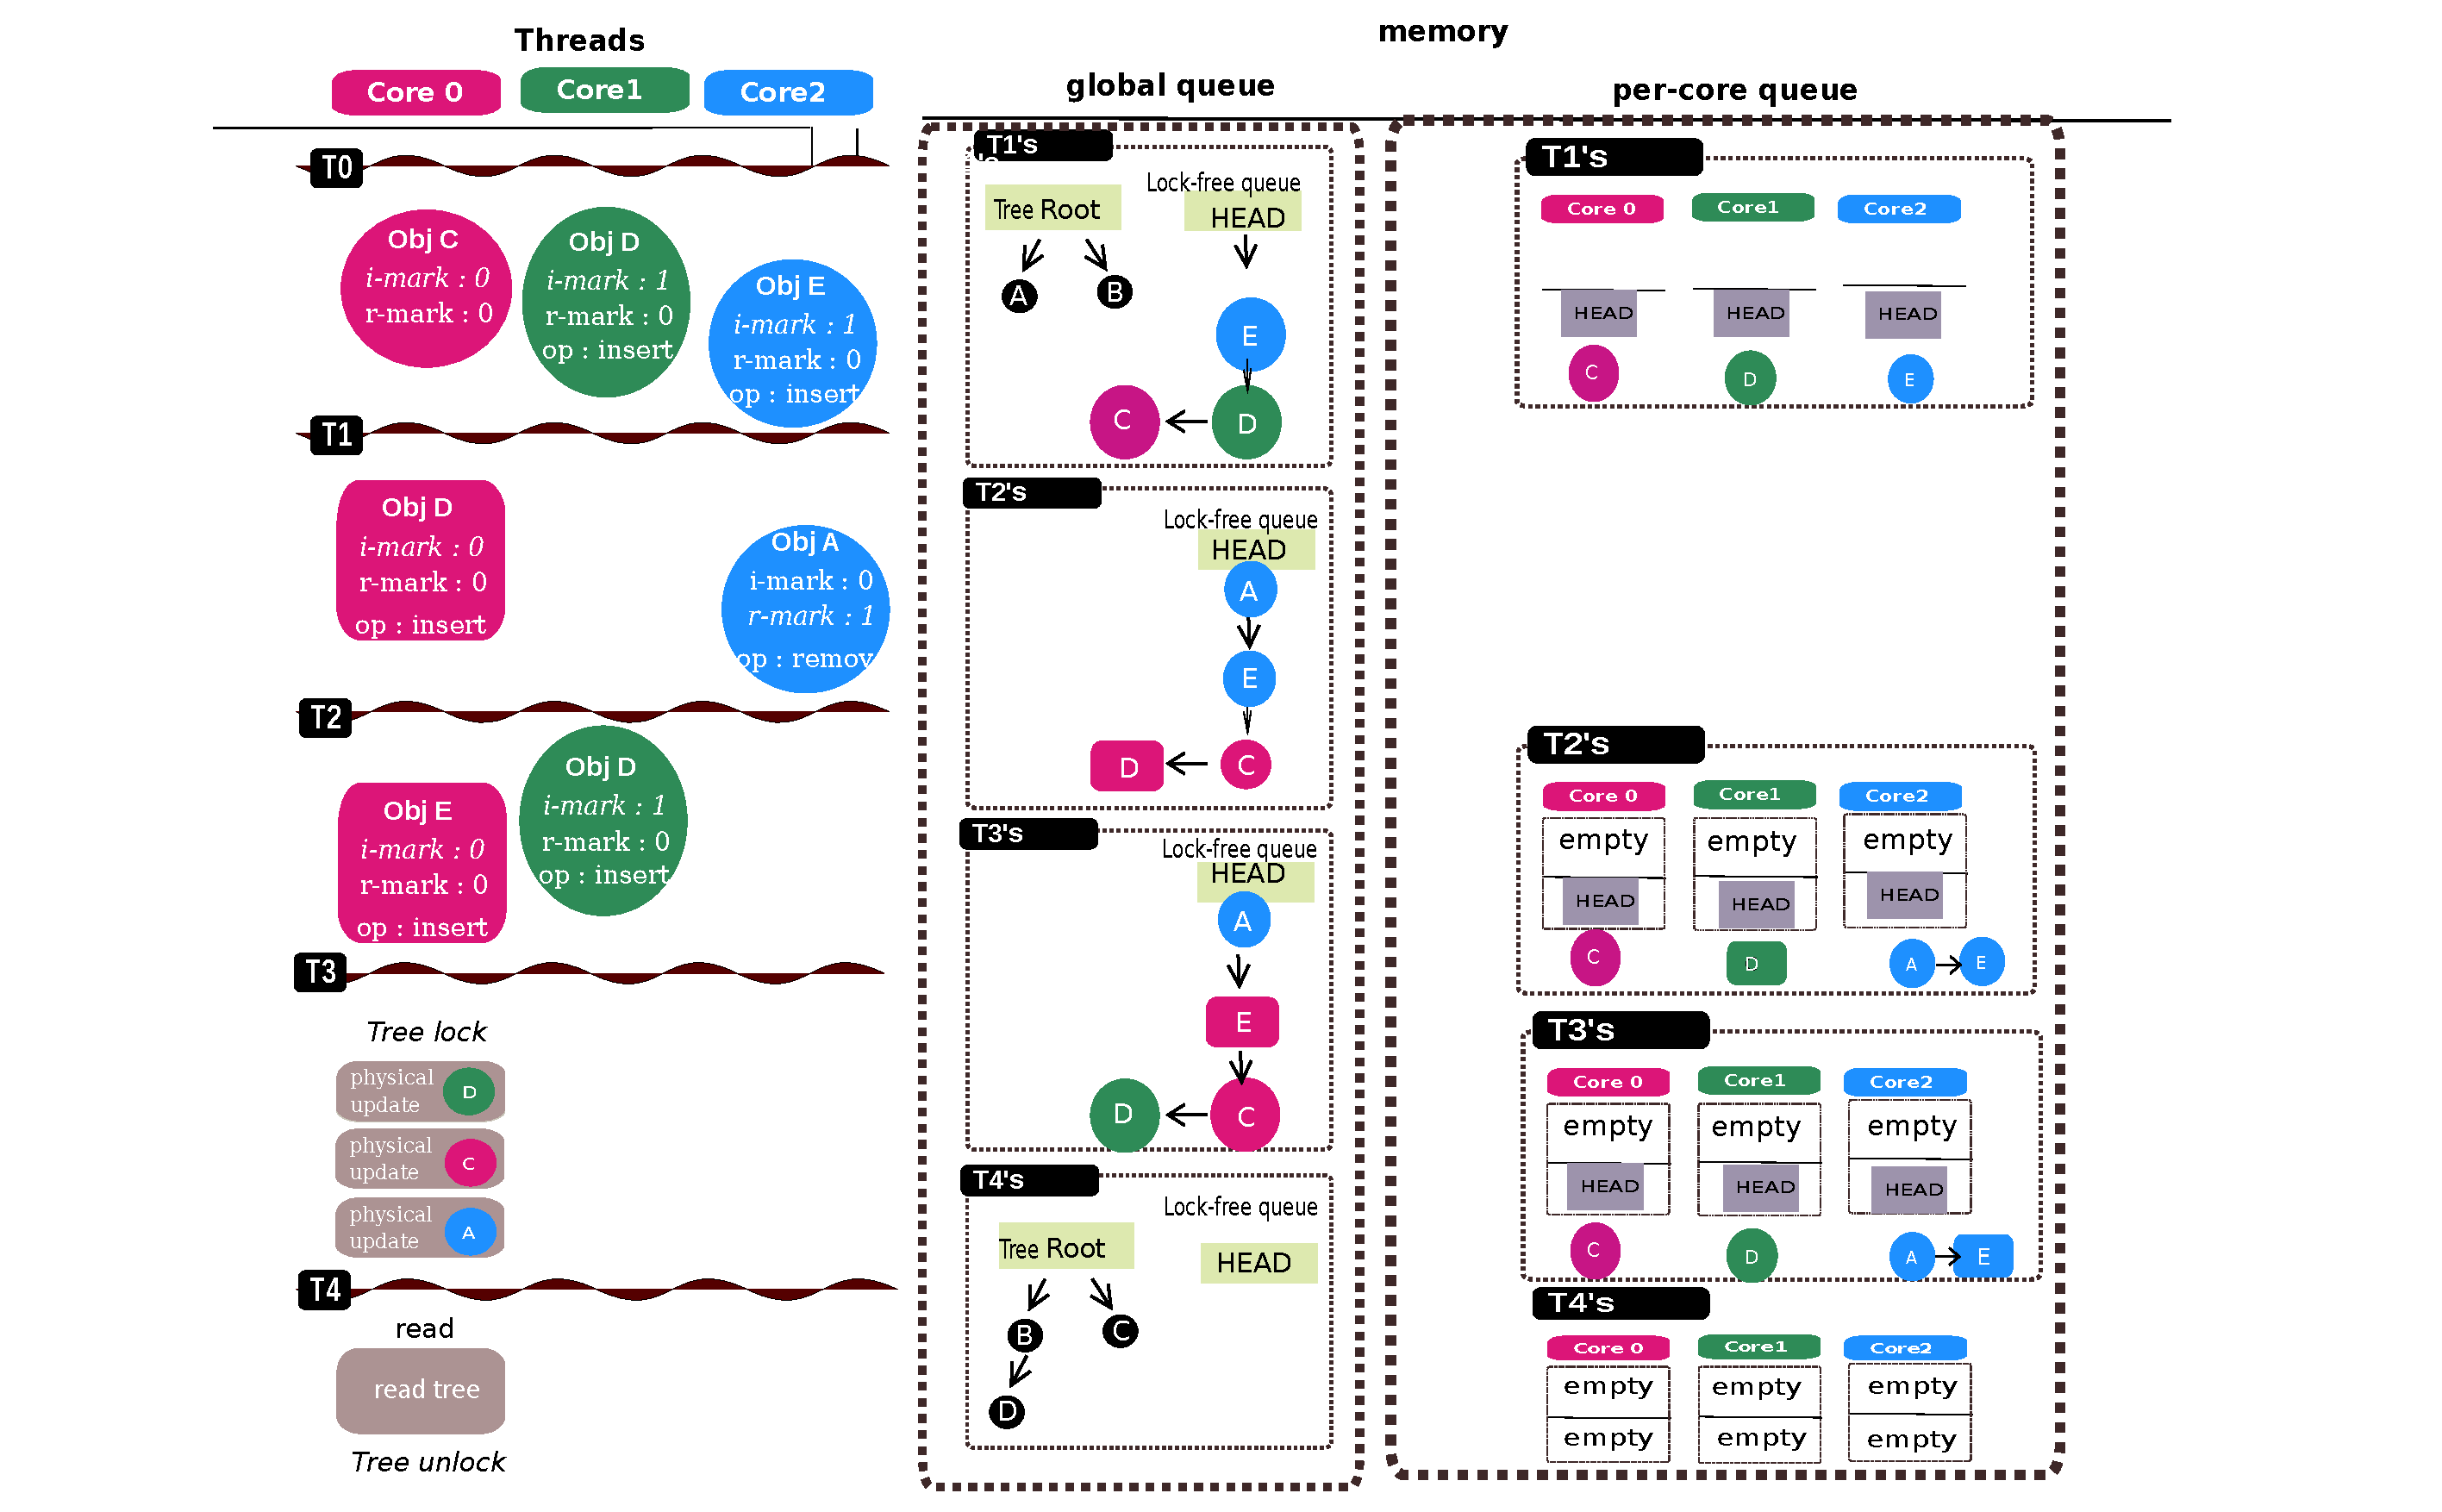
\includegraphics[width=1.0\textwidth,height=0.4\textheight]{fig/basic_gldu}
  \end{center}
  \caption{\deferu example showing six update operations and one read
  operation. The execution flows from top to bottom. Memory represents original
  data structure and logging queue at T1, T2 and T3, respectively.}
  \label{fig:basic}
\end{figure*}

%$$$$$$$$$$$$$$$$$$$$$$$$$$$$$$$$$$$$$$$$$$$$$$$$$$$$$$$$$$$$$$$$$$$$$$$$$$$$$$$$
%Paragraph 1-삭제 예정: LDU는 another log-based 기법 : read before physical update 
%$$$$$$$$$$$$$$$$$$$$$$$$$$$$$$$$$$$$$$$$$$$$$$$$$$$$$$$$$$$$$$$$$$$$$$$$$$$$$$$$

\ifkor
%LDU는 먼저 lock 없이 concurrent Updates를 수행하기 위해, update를 수행하는 시점에서 lock이 필요없는 방법으로
%operation log를 저장 한다.
%따라서 lock이 없이 짐에 따라 scalability가 뿐만 아니라 lock 자체의 오버헤를 줄일 수 있다.
%저장된 Log는 불필요한 메모리 낭비를 줄이기 위해 주기적으로 flush하거나 또는 read 전에 호출되게 되는데, 이 때 LDU는 FC와
%같이 operation Log를 corse grain lock과 함께 single core에서 sequntial 프로세싱을 통해 수행한다. 
%따라서 cache의 miss를 줄여 성능을 향상시킨다[].
%다음으로 LDU는 Log-based 방법과 같이 기존 data structure를 많이 수정하지 않고도 다른 data structure에 쉽게
%적용할 수 있다.
\else
%For update-heavy data structure LDU update before read operation;for example,
% it similar to CoW(Copy On Write) method because acture update as long as
% possible late.
\fi

%$$$$$$$$$$$$$$$$$$$$$$$$$$$$$$$$$$$$$$$$$$$$$$$$$$$$$$$$$$$$$$$$$$$$$$$$$$$$$$$$
%Paragraph 2: timestamp가 필요한 이유 : time-sensitive update operation log.
%$$$$$$$$$$$$$$$$$$$$$$$$$$$$$$$$$$$$$$$$$$$$$$$$$$$$$$$$$$$$$$$$$$$$$$$$$$$$$$$$
\ifkor
synchronized timestamp가 근본적으로 필요한 이유는 when a process logs an insert operation
on one core, migrates to another core, and logs a remove operation, the remove
should eventually execute after the insert[].
LDU는 update 순간 time-sensitive log를 제거함으로 synchronized timestamp counter 때문에 발생하는
문제를 해결하였다.
time-sensitive log란 순서가 바꿔서는 안되는 operation log이다. 
본 논문에서는 이러한 time-sensitive log를 설명하기 위해, ~\cite{Clements15SCR}에서 사용한 심볼방법을
이용하였다.
먼저 $\oplus$와 $\ominus$는 각각 insert와 remove update operation을 의미한다.
바로 따라오는 심볼은 object의 명을 의미하고 색깔과 높낮이는 서로 다른 CPU를 의미한다.
\begin{center}
$\oplus$\inv{1}{A}, $\oplus$\inv{2}{B}, $\oplus$\inv{3}{C},$\ominus$\inv{2}{A},
$\ominus$\inv{3}{C}, $\oplus$\inv{3}{A}, $\oplus$\inv{3}{C},$\ominus$\inv{1}{C}
\end{center}
즉 위와 같이 수행되었을 경우 time-sensitive log인 $\oplus$\inv{1}{A}과 $\ominus$\inv{2}{A}에
대해서는 항상 timestamp에 맞게 수행되어야 한다.
여기서 중요한 사실은 time-sensitive operation log은 삭제해도 괜찮은 operation log들 이다.
insert-remove operation 또는 remove-insert operation을 가지는 
$\ominus$\inv{2}{B}, $\oplus$\inv{3}{C} 삭제되도 괜찮으며, 결국 남은 operation log은 같은
object에 대해서 insert 또는 remove operation만 남게 된다.
위의 log는 아래와 같이 non-time-sensitive한 operation만 남게 된다.
\begin{center}
 $\oplus$\inv{2}{B}, $\oplus$\inv{3}{A}
\end{center}
LDU는 update-side removing이라는 방법으로 이러한 time-senstivive한 log를 update 순간 바로
지운다.
\else
%Synchronized timestamp가 근본적으로 필요한 이유는 when a process logs an insert operation
% on one core, migrates to another core, and logs a remove operation, the remove
% should eventually execute after the insert[].
The fundamental reason for requiring synchronized timestamp counters is that 
some operations should need to be ordered.
For example, a process logs an insert operation to per-core memory, then
migrates to another core, and logs a remove operation to per-core memory.
The remove operation must eventually execute after the insert operation[].
Thus, OpLog should needs synchronized timestamp counters.
%본 논문에서는 이러한 time-sensitive log를 설명하기 위해, ~\cite{Clements15SCR}에서 사용한 심볼방법을
% 이용하였다.
To explain this time-sensitive log, we use symbol label used by this
paper~\cite{Clements15SCR}.
%먼저 $\oplus$와 $\ominus$는 각각 insert와 remove update operation을 의미한다.
We describe insert as plus-circles $\oplus$, remove as minus-circles
$\ominus$ and object as color-circles \inv{2}{B}(object B). 
Color and vertical offset differentiate cpus.
%바로 따라오는 심볼은 object의 명을 의미하고 색깔과 높낮이는 서로 다른 CPU를 의미한다.
For example
\begin{center}
$\oplus$\inv{1}{A}, $\oplus$\inv{2}{B}, $\oplus$\inv{3}{C},$\ominus$\inv{2}{A},
$\ominus$\inv{3}{C}, $\oplus$\inv{3}{A}, $\oplus$\inv{3}{C},$\ominus$\inv{1}{C}
\end{center}
consists of five insert operations, three remove operation, three cpus, and
three objects.
%즉 위와 같이 수행되었을 경우 time-sensitive log인 $\oplus$\inv{1}{A}과 $\ominus$\inv{2}{A}에
% 대해서는 항상 timestamp에 맞게 수행되어야 한다.
This example show that $\oplus$\inv{1}{A} and $\ominus$\inv{2}{A},
time-sensitive log, must be executed in chronological order.
%LDU는 update 순간 이러한 time-sensitive log를 제거함으로 synchronized timestamp counter 때문에
% 발생하는 문제를 해결하였다.
LDU can eliminates this time-sensitive log when logs update operations with time
stamps, so LDU can removes synchronized timestamp counter.
%여기서 중요한 사실은 time-sensitive operation log은 삭제해도 괜찮은 operation log들 이다.
One more important fact that these time-sensitive operation logs may be removed
by optimization phase.
%예를 들어, insert-remove operation 또는 remove-insert operation을 가지는 
% $\ominus$\inv{2}{B}, $\oplus$\inv{3}{C} 삭제되도 괜찮으며, 결국 남은 operation log은 같은 object에 대해서 insert 또는
% remove operation만 남게 된다.
For example, insert-remove operations or remove-insert operations such as 
$\ominus$\inv{2}{B}, $\oplus$\inv{3}{C} are cancelable operations before
the read.
Eventually remaining operation logs such as
%위의 log는 아래와 같이 non-time-sensitive한 operation만 남게 된다.
\begin{center}
 $\oplus$\inv{2}{B}, $\oplus$\inv{3}{A}
\end{center}
, which are non-time-sensitive logs.
%LDU는 update-side removing이라는 방법으로 이러한 time-senstivive한 log를 update 순간 바로 지운다.
When updates operation occurs, LDU removes these time-sensitive log using
update-side removing technique.
\fi

%$$$$$$$$$$$$$$$$$$$$$$$$$$$$$$$$$$$$$$$$$$$$$$$$$$$$$$$$$$$$$$$$$$$$$$$$$$$$$$$$
%Paragraph 3:  time-sensitive update operation 삭제 방법: Update-side Abosrbing 
%$$$$$$$$$$$$$$$$$$$$$$$$$$$$$$$$$$$$$$$$$$$$$$$$$$$$$$$$$$$$$$$$$$$$$$$$$$$$$$$$

\ifkor
LDU는 time-senstivive한 log를 제거하기 위해 update-side removing이라는 방법을 사용한다.
이 방법은 만약 같은 object에 대해서 insert와 remove가 발생하였으면, 같은 object에
대해서, insert oepration과 remove operation에 대한 log를 update시점에 바로 바로 삭제하는 방법이다. 
syncronized timestamp counters 기반의 OpLog도 이러한 log 삭제 방법 수행하여 최적화를 하였으나,
operation log가 서로 다른 코어에 존재하는 log 같은 경우에 log를 merge와 검색한 후 삭제를 해야한다. 
syncronized timestamp counters 방법은 워크로드에 따라, 최적화를 위해 또 다른 sequntial 프로세싱이
요구된다.
하지만 LDU는 indivisual object를 대상으로 swap atomic operation을 사용하여
shared log 삭제하는 방법을 사용해서 이런 문제가 없다.
\else
%LDU는 time-senstivive한 log를 제거하기 위해 update-side removing이라는 방법을 사용한다.
%이 방법은 만약 같은 object에 대해서 insert와 remove가 발생하였으면, 같은 object에 대해서, insert
% oepration과 remove operation에 대한 log를 update시점에 바로 바로 삭제하는 방법이다.
To remove the time-senstivive log, LDU uses the update-side removing which is if
insert-remove operation occur in terms of same object, the same object's
insert-remove operation would be removed on the update time.
%syncronized timestamp counters 기반의 OpLog도 이러한 log 삭제 방법 수행하여 최적화를 하였으나,
% operation log가 서로 다른 코어에 존재하는 log 같은 경우에 log를 merge와 검색한 후 삭제를 해야한다.
%syncronized timestamp counters 방법은 워크로드에 따라, 최적화를 위해 또 다른 sequntial 프로세싱이 요구된다.
Indeed, the OpLog also optimizes by removing the existing operation rather than
adding the new one.
OpLog optimization is that becasue it may migrates other core, and then it logs
per-core memory, it needs to merge and search for removing the operation log,
which is additional sequntial processing for optimization.
%하지만 LDU는 indivisual object를 대상으로 swap atomic operation을 사용하여 shared log 삭제하는
% 방법을 사용해서 이런 문제가 없다.
LDU, however, have no problem migrating other core
\fi

%$$$$$$$$$$$$$$$$$$$$$$$$$$$$$$$$$$$$$$$$$$$$$$$$$$$$$$$$$$$$$$$$$$$$$$$$$$$$$$$$
%Paragraph 4: 리눅스의 update operation의 특징을 이용한 Update-side Abosrbing 
%$$$$$$$$$$$$$$$$$$$$$$$$$$$$$$$$$$$$$$$$$$$$$$$$$$$$$$$$$$$$$$$$$$$$$$$$$$$$$$$$
\ifkor
이처럼 log가 삭제될 수 있는 이유는 리눅스 커널의 operation은 순서가
있기 때문이다.
LDU는 insert operation 다음에는 반드시 remove opration이 발생하고 remove operation 다음에는 반드시
insert operation이 발생하는 특징을 이용하였다.
%이러한 data structure는 search에서 이미 필터링이 되기 때문
이러한 특징을 가지는 이유는 리눅스의 data structure의 경우에는 search와 update가 분리되어 있어, 같은 update
operation이 연달아 호출되지 않는다.
search가 two update operations(one to insert and one to remove an element)이 함수
외부해서 수행하는 구조이기 때문에 가능하다.
\else
%이처럼 update-side absorbing으로 log를 지울 수 있는 근본 이유는 리눅스 커널(freeBSD 커널 역시) search가
%two update operations(one to insert and one to remove an element)이 함수 외부해서 수행하는
%구조이기 때문에 가능하다.
To the best of our knowledge, LDU is the first log-based concurrent updates to
remove logs on the update time because we found that Linux kernel's updates
operations involved sequence of operations.
%예를 들어, 리눅스의 data structure 구조는 search가 update operaton 외부에 있기 때문에 insert
% operation 다음에는 반드시 remove opration이 발생하고 remove operation 다음에는 반드시 insert operation이
% 발생하는 특징이 있다. 
The Linux kernel, for example, if insert operation occur, then next operation
must be remove operation becasue the kernel's update function has separated
from search, alloc and free functions.
Therefore, remove-remove or insert-insert operation in Linux kernel is
forbidden: if remove-remove operation occur, the second remove operation may
encounter a crash because this object can be freed by first remove
operation concurrently.
%즉 리눅스의 data structure의 경우에는 search와 update가 분리되어 있어, 같은 update operation이 연달아
% 호출되지 않는다.
%LDU는 이러한 사실을 이용하여 update-side absorbing log를 개발 하였다. 
Therefore, the design of the LDU is inspired by these kernel update operations
sequeunce.
\fi

%$$$$$$$$$$$$$$$$$$$$$$$$$$$$$$$$$$$$$$$$$$$$$$$$$$$$$$$$$$$$$$$$$$$$$$$$$$$$$$$$
%Paragraph 4-1: CSDS 방법들 - 졸업논문
%$$$$$$$$$$$$$$$$$$$$$$$$$$$$$$$$$$$$$$$$$$$$$$$$$$$$$$$$$$$$$$$$$$$$$$$$$$$$$$$$

\ifkorthesis
이와 반대로 research 분야에서 많이 연구되는 CSDS(Concurrent search data
structures)~\cite{David2015ASYNCHRONIZED}의 방법들은 search가 update operation 내부에
존재하는 구조로 되어 있다.
따라서 같은 key값의 노드에 대해서 insert-insert 또는 remove-remove 순서로 동작할 수 있다.
이처럼 CSDS 알고리즘일 경우에는 LDU를 적용하지 못하는 limitation이 있다.
하지만 본 연구는 리눅스 커널과 같은 practical한 data structure에 초점을 맞추었기 때문에, 
research 분야에 많이 연구되고 있는 CSDS 알고리즘은 고려하지 않았다.
아직 CSDS의 non-blocking 알고리즘들은 garbage collector~\cite{AlBahra2013NAS},
iteration~\cite{petrank2013lock}, ordering~\cite{zhang2013practical}여러
practical한 이유로 C언어로 구현된 리눅스 커널 등에 적용하기에는 아직 한계가 있다.
\fi


%$$$$$$$$$$$$$$$$$$$$$$$$$$$$$$$$$$$$$$$$$$$$$$$$$$$$$$$$$$$$$$$$$$$$$$$$$$$$$$$$
%Paragraph 5: 리눅스의 Update-side removing 수행 방법
%$$$$$$$$$$$$$$$$$$$$$$$$$$$$$$$$$$$$$$$$$$$$$$$$$$$$$$$$$$$$$$$$$$$$$$$$$$$$$$$$
\ifkor
업데이트 순간 로그를 지우는 방법은 shared memory system의 swap operation을 사용한다.
이를 위해, LDU는 모든 object에 insert와 remove의 mark 필드를 추가해서 update-side
absorbing을 수행 하였다.
예를 들어 만약 A라는 object를 대상으로 insert-remove operation이 수행될 경우 처음 insert operation은
insert mark 필드에 표시하고 queue에 저장한다.
다음 remove operation 부터는 log를 queue에 저장하지 않고 insert에 표시한 mark 필드에 표시한 값만
atomic하게 지워주는 방식으로 진행된다.
다음으로 LDU는 log를 적용할 때, queue안에 log가 존재하더라도, mark 필드가 표시된 log만 실행한다.
이것은 swap이라는 상대적으로 가벼운 연산과 상대적으로 덜 share 하는 indivisaul global object의 mark filed를
사용해서 time-sensitive한 operation을 제거할 뿐만 아니라, 동시에 실제 operation을 수행하지 않고 log를 지워주는
효과를 가져주므로 성능이 향상된다. 
\else
%업데이트 순간 로그를 지우는 방법은 shared memory system의 swap operation을 사용한다.
Update-side removing logs are implemented by performing atomic swap operation
in an individual object for shared memory systems.
%이러한 atomic swap operation은 update operation을 취소 가능한 로그와 함께 atomic하게 삭제하는 일을
% 가능하게 한다.
This atomic swap operation alows update operations to atomically remove with the
previous cancelable log.
%먼저 LDU는 모든 object에 insert와 remove의 mark 필드를 추가해서 update-side absorbing을 수행
% 하였다.
To that these LDU performs adding the marking field in the object structure.
%예를 들어 만약 A라는 object를 대상으로 insert-remove operation이 수행될 경우 처음 insert operation은
% insert mark 필드에 표시하고 queue에 저장한다.
For example, consider the insert-remove operation sequence at same object.
The first insert operation marks the feld of mark and then the log inserts
queue.
%다음 remove operation 부터는 log를 queue에 저장하지 않고 insert에 표시한 mark 필드에 표시한 값만
% atomic하게 지워주는 방식으로 진행된다.
After the next remove operation, LDU does not logs and proceed with changing
the mark feld.
%다음으로 LDU는 log를 적용할 때, queue안에 log가 존재하더라도, mark 필드가 표시된 log만 실행한다.
The reader applies logs, marking feld is true, to the original data structure.
%이것은 swap이라는 상대적으로 가벼운 연산과 상대적으로 덜 share 하는 indivisaul global object의 mark
% filed를 사용해서 time-sensitive한 operation을 제거할 뿐만 아니라, 동시에 실제 operation을 수행하지 않고
% log를 지워주는 효과를 가져주므로 성능이 향상된다. 
The benefit of this update-side removing is twofold:not only it can eliminates
the time-sensitive operation but also it can cancels the previous operation log
in the queue with current operation.
\fi

%$$$$$$$$$$$$$$$$$$$$$$$$$$$$$$$$$$$$$$$$$$$$$$$$$$$$$$$$$$$$$$$$$$$$$$$$$$$$$$$$
%Paragraph 7: 또 최적화 방법 reusing garbage object : 
%$$$$$$$$$$$$$$$$$$$$$$$$$$$$$$$$$$$$$$$$$$$$$$$$$$$$$$$$$$$$$$$$$$$$$$$$$$$$$$$$

\ifkor
LDU의 또 다른 최적화 기법은 update-side removing 때문에 취소된 garbage log를 재활용하는 것이다.
이 garbage log는 queue에는 존재하지만 update-side aborsrbing 때문에 취소 되어 garbage가 되어 queue에
보관되어 있는 log이다. 
이러한 garbage log일 경우 다음 update operation에 대해서는 해당 로그를 새로 많들어 넣지 않고 기존 로그를 재활용하는
방법이다.
예를 들어 A라는 오브젝트에 대해서 insert-remove-insert 순서로 update가 수행될 경우, 세번째 insert 명령어는
queue에 들어가 있지만 update-side absorbing 때문에 최소되어 insert mark filed가 zero인
경우(garbage object)이다.
이러한 경우, 다음 insert operation에 대해서는 새로운 log를 list에 연산으로 다시 넣지 않고, 해당 object의 mark
필드만 변경하여 log를 재활용하는 방법을 사용한다.
\else
%LDU의 또 다른 최적화 기법은 garbage log를 재활용하는 것이다.
%이 garbage log는 queue에는 존재하지만 update-side removing 때문에 취소 되어 garbage가 되어
% queue에 보관되어 있는 log이다. 
The second technique, called reusing garbage logs, reuse garbage log without
creating new log.
The garbage log aleady canceled through the update-side removing, but it
remained queue.
%예를 들어 A라는 오브젝트에 대해서 insert-remove-insert 순서로 update가 수행될 경우, 세번째 insert 명령어는
% queue에 들어가 있지만 update-side absorbing 때문에 최소되어 insert mark filed가 zero인
% 경우(garbage object)이다.
For example, consider the insert-remove-insert operation.
After the sencond remove operation, the log remained in the queue, but it
already canceled log resulted from update-side removing, hence insert mark filed is
zero in the queue.
%이러한 경우, 다음 insert operation에 대해서는 새로운 log를 list에 연산으로 다시 넣지 않고, 해당 object의 mark
% 필드만 변경하여 log를 재활용하는 방법을 사용한다.
In this case, the third insert operation reuse log in the queue instead of 
creating a new log using atomic swap, so it not only reduce memory overhead but
also remove queueing overhead.
\fi

%$$$$$$$$$$$$$$$$$$$$$$$$$$$$$$$$$$$$$$$$$$$$$$$$$$$$$$$$$$$$$$$$$$$$$$$$$$$$$$$$
%Paragraph 8: LDU의 로그는 두 종류의 queue에 저장할 수 있도록 지원
%$$$$$$$$$$$$$$$$$$$$$$$$$$$$$$$$$$$$$$$$$$$$$$$$$$$$$$$$$$$$$$$$$$$$$$$$$$$$$$$$
\ifkor
LDU는 보다 다양한 데이터 구조를 지원하기 위해, per-core 또는 global queue 모두 이용할 수 있게 설계하였다.
그 이유는 데이터 구조가 특성에 따라 per-core 구조에 적당한 data structure가 있고,
global queue 구조에 적당한 데이터 구조가 있기 때문이다.
먼저 LDU의 Per-core queue는 queue에 log를 저장할 때, global head 포인터에 대한 CAS operation을
완전히 제거한 장점을 가진다.
LDU의 per-core queue에 대한 단점으로는 time-senstivive log가 제거되었더라도,
앞에서 설명한 예와 같이 남은 로그들인 $\oplus$\inv{2}{B}, $\oplus$\inv{3}{A}는 순서가 바뀔 수 있다.
이러한 경우 tree와 같은 data structure는 문제가 없으나, stack과 같이 남은 operation의
순서도 민감한 data structure는 사용하지 못하는 문제점이 있다.
또한 전형적인 per-core queue를 방법의 단점으로 메모리 관리 코드에 대한 복잡도가 증가되고, 
메모리 사용량도 per-core에 추가적으로 할당을 받으므로 증가된다.
이를 보완하기 위해 LDU는 global queue도 같이 지원한다.
LDU의 global queue의 장점은 광장히 simple하여 어떻한 data structure라도 쉽게 적용이 가능하다.
또한 per-core 처럼 global head포인터에 대한 CAS연산을 완전히 제거하지 못하지만, LDU의 update-side
removing log와 reuse garbage log 기법등으로 global queue에 log를 저장하는 횟수를 상당히 줄임에 따라,
cache communication overhead를 상당히 줄일 수 있다.
\else
%LDU는 보다 다양한 데이터 구조를 지원하기 위해, per-core 또는 global queue 모두 이용할 수 있게 설계하였다.
We designs using per-core and global queue for saving the logs becasue it
can the further support of various data structure.
%그 이유는 데이터 구조가 특성에 따라 per-core 구조에 적당한 data structure가 있고,
%global queue 구조에 적당한 데이터 구조가 있기 때문이다.
If per-core queue does not properly apply to a data structure, may use the
global queue to reduce the drawback of the per-core queue.
%먼저 LDU의 Per-core queue는 queue에 log를 저장할 때, global head 포인터에 대한 CAS operation을
%완전히 제거한 장점을 가진다.
The per-core queue of the LDU can remove CAS operations that access global head
pointer when logs update operation. 
%LDU의 per-core queue에 대한 단점으로는 time-senstivive log가 제거되었더라도,
%앞에서 설명한 예와 같이 남은 로그들인 $\oplus$\inv{2}{B}, $\oplus$\inv{3}{A}는 순서가 바뀔 수 있다.
However, although LDU removes time-sensitive log, 
%이러한 경우 tree와 같은 data structure는 문제가 없으나, stack과 같이 남은 operation의
%순서도 민감한 data structure는 사용하지 못하는 문제점이 있다.
the LDU can not apply more time-sensitive data structures such as stack and
queue because these data structures corresponding characteristic
%또한 전형적인 per-core queue를 방법의 단점으로 메모리 관리 코드에 대한 복잡도가 증가되고, 
%메모리 사용량도 per-core에 추가적으로 할당을 받으므로 증가된다.
In addition, per-core queue memort usage is high.
%이를 보완하기 위해 LDU는 global queue도 같이 지원한다.
To overcome these shortcomings, LDU also supports the global queue.
%LDU의 global queue의 장점은 광장히 simple하여 어떻한 data structure라도 쉽게 적용이 가능하다.
The global queue of LDU is simple and easy, so it can use any data structure.
%또한 per-core 처럼 global head포인터에 대한 CAS연산을 완전히 제거하지 못하지만, LDU의 update-side
%removing log와 reuse garbage log 기법등으로 global queue에 log를 저장하는 횟수를 상당히 줄임에 따라,
%cache communication overhead를 상당히 줄일 수 있다.
Though global queue can not perfactly remove global CAS operations, it can
reduce cache communication overhead by using update-side removing
logs and reuse garbage logs because it reduces count of inserting the
queue.
\fi

%$$$$$$$$$$$$$$$$$$$$$$$$$$$$$$$$$$$$$$$$$$$$$$$$$$$$$$$$$$$$$$$$$$$$$$$$$$$$$$$$
%Paragraph 9: log를 저장하는 queue의 종류는 non-blocking queue를 사용
%$$$$$$$$$$$$$$$$$$$$$$$$$$$$$$$$$$$$$$$$$$$$$$$$$$$$$$$$$$$$$$$$$$$$$$$$$$$$$$$$
\ifkor
LDU는  non-blocking queue를 이용하여 로깅한다. 그 이유는 Global 또는 Per-core 락 없이 수행될 수 
있기 때문이다. 
Non-blocking queue 중에 LDU는 head 포인터에 대한 CAS 연산을 최대한 줄인 multiple producers and
single consumer에 활용될 수 있는 자료구조[]를 이용하였다.
이 큐는 다른 non-blocking list[][][]와 다르게, insert operation을 항상 처음 노드에 삽입함에
따라, CAS가 발생되는 횟수를 상대적으로 줄일 수 있다.
게다가 log를 적용하는 부분에서 single consumer만 고려 했기 때문에, remove를 위한 복잡한 알고리즘이 필요없다. 
예를 들어 single consumer는 operation log 전체를 얻기 위해, xchg 명령을 사용하여 head pointer를
NULL로 atomic하게 제거한다. 
\else
%LDU는  non-blocking queue를 이용하여 로깅한다. 그 이유는 Global 또는 Per-core 락 없이 수행될 수 
%있기 때문이다. 
LDU logs in non-blocking queue because it can proceed without any lock(per-core
or global lock).
%Non-blocking queue 중에 LDU는 head 포인터에 대한 CAS 연산을 최대한 줄인 multiple producers and
%single consumer에 활용될 수 있는 자료구조[]를 이용하였다.
Among non-blocking queues, the LDU uses multiple producers and single consumer
based non-blocking queue reducing the CAS operationg to global head pointers
access.
%이 큐는 다른 non-blocking list[][][]와 다르게, insert operation을 항상 처음 노드에 삽입함에
%따라, CAS가 발생되는 횟수를 상대적으로 줄일 수 있다.
This queue always inserts node where inserts head-next pointer, so it can
reduce iteration loop that may make anonther CAS operation.
%게다가 log를 적용하는 부분에서 single consumer만 고려 했기 때문에, remove를 위한 복잡한 알고리즘이 필요없다. 
In addition, this queue considers single consumer when applying logs, so it does
not need complex algorithms for the remove oepration.
%예를 들어 single consumer는 operation log 전체를 얻기 위해, xchg 명령을 사용하여 head pointer를
%NULL로 atomic하게 제거한다. 
For example, this queue uses atomic SWAP operation, which changes NULL pointer,
to acquire all operating log.
\fi

%$$$$$$$$$$$$$$$$$$$$$$$$$$$$$$$$$$$$$$$$$$$$$$$$$$$$$$$$$$$$$$$$$$$$$$$$$$$$$$$$
%Paragraph 11: 중간에 한번씩 log를 flush
%$$$$$$$$$$$$$$$$$$$$$$$$$$$$$$$$$$$$$$$$$$$$$$$$$$$$$$$$$$$$$$$$$$$$$$$$$$$$$$$$

\ifkor
LDU는 log 때문에 불필요하게 메모리 낭비를 방지하고, To keep the log from growing without end,
log-based method periodically apply the time-ordered operations at the head of
the log to remove these opearation from the log.
LDU는 주기적으로 Log를 적용함으로 Log가 쌓여서 발생하는 메모리 낭비를 줄인다. 
이것은 OpLog의 batching updates와 Flat combining의 combiner thread와 같이, 1개의
thread가 update operation을 수행하므로 cache locality가 높아지는 장점을 가진다. 
\else
%LDU는 log 때문에 불필요하게 메모리 낭비를 방지하고, To keep the log from growing without end,
%log-based method periodically apply the time-ordered operations at the head of
% the log to remove these opearation from the log.
To reduce memory usage and to keep the log from growing without end, LDU
periodically apply the time-ordered operations at the head of the log to remove
these opearation from the log.
%LDU는 주기적으로 Log를 flush해줌으로써 Log가 쌓여서 발생하는 메모리 낭비를 줄인다.
The LDU periodically applies logs in queue to reduce the memory overhead.
%이것은 OpLog의 batching updates와 Flat combining의 combiner thread와 같이, 1개의
%thread가 update operations을 수행하므로 cache locality가 높아지는 장점을 가진다. 
This approch is similar with the method of previous research such as OpLog's
batching updates and FC's combiner thread.

\fi


%$$$$$$$$$$$$$$$$$$$$$$$$$$$$$$$$$$$$$$$$$$$$$$$$$$$$$$$$$$$$$$$$$$$$$$$$$$$$$$$$
%$$$$$$$$$$$$$$$$$$$$$$$$$$$$$$$$$$$$$$$$$$$$$$$$$$$$$$$$$$$$$$$$$$$$$$$$$$$$$$$$
%$$$$$$$$$$$$$$$$$$$$$$$$$$$$$$$$$$$$$$$$$$$$$$$$$$$$$$$$$$$$$$$$$$$$$$$$$$$$$$$$
%$$$$$$$$$$$$$$$$$$$$$$$$$$$$$$$$$$$$$$$$$$$$$$$$$$$$$$$$$$$$$$$$$$$$$$$$$$$$$$$$


\subsection{LDU example}


%$$$$$$$$$$$$$$$$$$$$$$$$$$$$$$$$$$$$$$$$$$$$$$$$$$$$$$$$$$$$$$$$$$$$$$$$$$$$$$$$
%Paragraph 1: Flowchart 구조 설명 
%$$$$$$$$$$$$$$$$$$$$$$$$$$$$$$$$$$$$$$$$$$$$$$$$$$$$$$$$$$$$$$$$$$$$$$$$$$$$$$$$
%
\ifkor
그림 \ref{fig:basic} LDU의 하나의 예에 대해서 보여준다. 그림 \ref{fig:basic}은 예로서 queue를 global
queue를 사용하였다. 
7개의 update operation과 1개의 read operation을 LDU에서 어떻게 처리하는지 보여준다.
update operation에 대해서는 앞에서 설명한 심볼을 사용했고 garbage object을 위한 심볼이 추가 되었다.
garbage object는 \res{1}{D}과 같이 rectangle로 표시한다. 
이 그림의 실행 순서는 위에서 부터 아래이다.
그림의 왼쪽은 CPU의 operation 순서를 보여주고 오른쪽은 특정 시간에 메모리에 저장된 자료구조의 내용을 보여준다.
초기 data structure의 트리에는 \inv{0}{A} and \inv{0}{B} 두개의 오브젝트가 들어가고, global
queue에는 아무것도 없다.
\else
%그림 \ref{fig:basic} LDU의 하나의 예에 대해서 보여준다. 그림 \ref{fig:basic}은 예로서 queue를 global
%queue를 사용하였다. 
Figure \ref{fig:basic} shows an example of the LDU with a per-core queue and
a global queue.
%LUD는 update-heavy한 자료구조를 해결하였기 때문에 우리는 7개의 update operation과 1개의 read
% operation을 LDU에서 어떻게 처리하는지 보여준다.
Becuase LDU can solve update-heavy data structure, we show how six update
operations can concurrently run without lock before the read operation.
%update operation을 위한 심볼은 앞에서 설명한 심볼인 사용했고 garbage object을 위한 심볼이 추가 되었다.
%garbage object는 \res{1}{D}과 같이 rectangle로 표시한다. 
To explain the LDU, we previously used symbol and add garbage symbol as
rectangle \res{1}{D}.
%이 그림의 실행 순서는 위에서 부터 아래이다.
In this figure, execution flows from top to bottom.
%그림의 왼쪽은 CPU의 operation 순서를 보여주고 오른쪽은 특정 시간에 메모리에 저장된 자료구조의 내용을 보여준다.
The left box show cpu operation, and the right box show data structure
contents at a particular time in the memory.
%초기 data structure의 트리에는 \inv{0}{A} and \inv{0}{B} 두개의 오브젝트가 들어가고, global
%queue에는 아무것도 없다.
Early the tree data structure contains two object, \inv{0}{A} and \inv{0}{B},
and queue is empty.
\fi

%$$$$$$$$$$$$$$$$$$$$$$$$$$$$$$$$$$$$$$$$$$$$$$$$$$$$$$$$$$$$$$$$$$$$$$$$$$$$$$$$
%Paragraph 2: Flowchart 그림 설명 
%$$$$$$$$$$$$$$$$$$$$$$$$$$$$$$$$$$$$$$$$$$$$$$$$$$$$$$$$$$$$$$$$$$$$$$$$$$$$$$$$
%
\ifkor
가장 위의 그림에서는  \code{Core0}, \code{Core1} and
\code{Core2}가 각각 $\oplus$\inv{1}{C}, $\oplus$\inv{2}{D} and
$\oplus$\inv{3}{E}에 해당하는 3개의 updates oepration을 락 없이 concurrent한 방법으로 log를 저장한다.
Log를 저장하는 queue를 non-blocking queue를 사용하기 때문에, 이 단계에서의 update는 lock이 필요없다. 
즉 모든 thread는 lock에 대한 contention없이 병렬적으로 실행된다. 
\code{T1} 시점이 되면 메모리의 트리는 \inv{0}{A} and \inv{0}{B}의 노드를 가지게 되고, queue에는 
$\oplus$\inv{1}{C}, $\oplus$\inv{2}{D} and $\oplus$\inv{3}{E}가 insert mark 필드가
true로 된 상태로 저장되어 있다. 
update-side absorbing 단계에서는  $\ominus$\inv{1}{D}명령이 수행되면, 새로운 object를 queue에 넣지
않고, mark 필드만 atomic하게 true로 수정한다.  
만약 처음 수행되는 $\ominus$\inv{3}{A} operation이면 queue에 넣는다.
\code{T2} 시점이 되면 메모리의 트리는 변함없고, queue에는 
$\oplus$\inv{1}{C}, $\oplus$\res{2}{D}, $\oplus$\inv{3}{E} and 가
$\ominus$\inv{3}{A} 저장된다. 여기서 \res{2}{D}는 mark필드가 false로 되어 garbage가 된 object이다.
reuse garbage log 단계에서는 \res{2}{D}와 같이 queue에는 들어가 있지만, garbage object인 경우 새롭게
queue에 operation log를 넣지 않고, mark 필드 변경으로 재사용하는 것이다. 
따라서 \res{2}{D}는 \inv{2}{D} 상태로 변경된다. 
\code{T3} 시점이 되면 queue에는 
$\oplus$\inv{1}{C}, $\oplus$\inv{2}{D}, $\oplus$\res{3}{E} and 가
$\ominus$\inv{3}{A} 저장된다.
마지막 단계인 저장된 log를 실행하는 단계에서는 tree에서 사용한 방법으로 lock를 건후 하나의 코어에서 
전체 로그를 update한다. 여기서 garbage log인  $\oplus$\inv{2}{D}을 제외하고 queue에 저장된 순서대로 
$\oplus$\inv{1}{C},$\oplus$\res{3}{E} and 가 $\ominus$\inv{3}{A}의 operation을
수행한다. \code{T4} 시점이 되면 tree에는 
모든 operation이 수행되어, \inv{0}{B}, \inv{0}{C} and \inv{0}{D} 값이 존재하게 된다.
결국 로그를 모두 수행하면 마지막 reader는 같은 tree의 값을 읽게 된다. 
\else
%가장 위의 그림에서는  \code{Core0}, \code{Core1} and
%\code{Core2}가 각각 $\oplus$\inv{1}{C}, $\oplus$\inv{2}{D} and
%$\oplus$\inv{3}{E}에 해당하는 3개의 updates oepration을 락 없이 concurrent한 방법으로 log를
% 저장한다.
The data structure for \emph{physical update} is a tree, and initial values in
the tree are node \code{A} and \code{B}.
In contrast, the data structure for \emph{logical update} is lock-less list.
In the top figure, \code{Core0}, \code{Core1} and \code{Core2} perform the
logical insert operation to nodes \code{C}, \code{D} and \code{E},
 respectively.
The logical inserts set the insert mark, and they then insert their
nodes into lock-less list.
In this case, none of the lock is needed because \deferu uses the lock-less
list;all threads can execute the update concurrently.
At \code{T1}, the tree contains node \code{A}
and \code{B} and 
the lock-less list contains node \code{E}, \code{D} and \code{C}.
When removing the node \code{C}, the node \code{C}, whose mark field was marked
by insert, atomically cleans up the insert marked field.
At \code{T2}, the lock-less list contains nodes
\code{A}, \code{E}, \code{D}, and \code{C}, and the marking field is zero for 
nodes \code{E} and \code{C}.
Before running the \code{synchronize} function, they need to lock the original
 tree's lock using the exclusive lock in order to protect the tree's
 operation.
The \code{synchronize} migrates from lock-less list node to tree node, each of 
which is the marked node, so nodes \code{A} and \code{D} are migrated.
Finally, the tree contains nodes \code{D} and \code{B}, so the reader can read
 eventually consistent data.
\fi

\subsection{The LDU Algorithm and Correctness}

\begin{figure}[tb]
\begin{center}
\inputminted[linenos,fontsize=\footnotesize, tabsize=2]{c}{src/ldu_logical.c}
\end{center}
\rule{\columnwidth}{0.5pt}
\vspace{-\baselineskip}
\caption{\deferu logical update algorithm. \code{logical\_insert} represents
 non-blocking insert function.
It may be called by original insert position without locks. The fastpath is
 that when their object was removed by \code{logical\_remove},
 \code{logical\_insert} just changes node's marking field.}
\label{fig:gldulogicalupdate}
\end{figure}

\begin{figure}[tb]
\begin{center}
\inputminted[linenos,fontsize=\footnotesize, tabsize=2]{c}{src/ldu_physical.c}
\end{center}
\rule{\columnwidth}{0.5pt}
\vspace{-\baselineskip}
\caption{\deferu physical update algorithm. \code{synchronize\_ldu} may be
 called by reader and converts update log to original data structure
 traversing the lock-less list.}
\label{fig:glduphysicalupdate}
\end{figure}

\subsubsection{logical update: inserting logs}
%$$$$$$$$$$$$$$$$$$$$$$$$$$$$$$$$$$$$$$$$$$$$$$$$$$$$$$$$$$$$$$$$$$$$$$$$$$$$$$$$
%Paragraph 1:LDU Concurrent Updates 알고리즘 코드 및 설명 
%$$$$$$$$$$$$$$$$$$$$$$$$$$$$$$$$$$$$$$$$$$$$$$$$$$$$$$$$$$$$$$$$$$$$$$$$$$$$$$$$
\ifkor
그림 \ref{fig:gldulogicalupdate}는 concurrent updates를 수행하는 코드와 앞에서 설명한 update-side
absorbing logs와 reuse garbage logs에 대한 코드이다. 
\code{logical\_insert}과 \code{logical\_remove}의 코드에서 가장 먼저하는 것은 이미 update
operation이 수행되어 log가 queue에 들어 있는지에 대해서 체크를 한다. 
이것은 update함수가 수행하는 도중 어느때나 log를 flush하는 \code{synchronize} 함수가 수행 될 수 있기 때문에,
\code{xchg} 함수를 통해 atomic하게 체크를 한다. 
또한 \code{xchg}를 통해 old mark 필드가 true라면 이미 queue에 log가 있다는 뜻이므로, atomic하게 false로
수정을 한다.
이것은 앞에서 설명한 update-side absorbing log 기능이며, 1개의 atomic operation으로 update를 수행할 수
있다.
만약 mark 필드카 체크되지 않았다면, 두번째로 queue에 존재하는 로그인지 체크를 한 후, 존재하는 로그라면
이미 앞에서 mark필드를 설정하여 이미 로그를 재활용했으므로 queue에 로그를 넣지 않는다.
만약 처음 사용된 log라면 non-blocking queue에 넣는다.
이 코드는 항상 옳게 동작한다.  
그 이유는 리눅스 update operation이 항상 insert-remove 순서나 remove-insert 순서로 실행되기 때문이다.
%만약 순서가 insert-insert 또는 remove-remove로 동작하면 
\else


\fi


\subsubsection{synchronize update: applying logs}


%$$$$$$$$$$$$$$$$$$$$$$$$$$$$$$$$$$$$$$$$$$$$$$$$$$$$$$$$$$$$$$$$$$$$$$$$$$$$$$$$
%Paragraph 2:LDU Deferred Updates 알고리즘 코드 및 설명 
%$$$$$$$$$$$$$$$$$$$$$$$$$$$$$$$$$$$$$$$$$$$$$$$$$$$$$$$$$$$$$$$$$$$$$$$$$$$$$$$$

\ifkor
그림 \ref{fig:glduphysicalupdate}는 concurrent updates를 통해 저장된 log들을 적용하는 deferred
update 함수에 대한 코드이다.
\code{synchronize\_ldu}는 마치 CoW 처럼 read 전에 호출되기도 하지만, 로그가 쌓이는것을 방지하기 위해 주기적으로
호출되어 로그를 비워준다.
이 함수는 항상 object의 lock이 걸린 상황에서 수행된다. 
LDU는 single consumer가 독점적으로 log를 처리한다.
%multiple-producer and/or multiple-consumer (MP/MC) variants.
따라서 제일 먼저 하는일은 queue에 저장된 log를 얻기 위해 atomic xchg operation으로 log의 head 포인터를
얻는다.
그리고 이 순간 부터는 single consumer가 독점적으로 log를 처리하게 된다.
LDU는 주기적으로 log를 비워줘야 하므로, update operation이 수행되는 도중에도 \code{synchronize\_ldu}가
호출될 수 있다.
따라서 항상 origianl data structure에 적용하기 전에 mark 필드를 초기화해야한다.
또한 log를 사용했으면, used 비트를 초기화 하여 해당 log가 queue 없음을 표시한다.
하지만 mark 필드 초기화 과정과 used 비트를 초기화 하는 과정에서, reuse garbase logs 기능 때문에,
언제든지 다시 concurrent updates operation을 통해 mark 필드가 설정될 수 있다.
따라서 한번 더 mark 필드를 체크하여 log를 비워준다.
\else

\fi

\ifkorthesis
%$$$$$$$$$$$$$$$$$$$$$$$$$$$$$$$$$$$$$$$$$$$$$$$$$$$$$$$$$$$$$$$$$$$$$$$$$$$$$$$$:w
% Thesis :
% Paragraph 2:LDU queue 알고리즘 코드 및 설명 - 졸업논문
%$$$$$$$$$$$$$$$$$$$$$$$$$$$$$$$$$$$$$$$$$$$$$$$$$$$$$$$$$$$$$$$$$$$$$$$$$$$$$$$$
\subsubsection{LDU queues}
\begin{figure}[tb]
\inputminted[linenos,fontsize=\footnotesize, tabsize=2]{c}{src/ldu_queue.c}
\rule{\columnwidth}{0.5pt}
\vspace{-\baselineskip}
\caption{\deferu physical update algorithm. \code{synchronize\_ldu} may be
 called by reader and converts update log to original data structure
 traversing the lock-less list.}
\label{fig:lduqueue}
\end{figure}

LDU의 로그를 저장하기 위한 2가지 queue에 대한 코드는 그림 \ref{fig:lduqueue}와 같다. 
앞에서 설명했듯이 LDU는 어떤 queue를 사용해도 문제 없도록 설계하였다.
따라서 queue 대한 의존성이 없다.
global queue를 사용할 경우 LDU는 항상 head의 first 포인터에 CAS연산으로 성공할 때까지 반복 수행 후 데이터를 넣는다. 
per-core queue를 사용할 경우는 per-core의 hash 테이블을 가지고 온 후 hash 테이블이 넣으려는 log의
data structure와 같은지 체크하고, 다르면 해당 코어에 저장된 log를 lock과 함께 update를 수행한다.
전체 코어의 log를 flush할 필요없이 해당 코어에 저장된 log만 flush하면 되는 이유는 이미 update-side
absorbing에 의해 time-sencitive한 operation이 삭제되었기 때문이다.
\fi


%$$$$$$$$$$$$$$$$$$$$$$$$$$$$$$$$$$$$$$$$$$$$$$$$$$$$$$$$$$$$$$$$$$$$$$$$$$$$$$$$
%Reference Sentence 1
%$$$$$$$$$$$$$$$$$$$$$$$$$$$$$$$$$$$$$$$$$$$$$$$$$$$$$$$$$$$$$$$$$$$$$$$$$$$$$$$$

%To keep the log from growing without end, we can at any point apply in-order a
%subsequence of the operations at the head of the log to the state to derive a
%new state, and remove these operation from the log[EuroSys 2006 PLS].

%High level operations performed on shared data structures can be divided into
%three groups: read-only, write-only, and read-modify-write[PLS].

%Read-only operations do not mutate the data, write-only operations modify the
%data but do not return a result, and read-modify-write operations change shared
%data and return a result that is dependent on the data read[PLS].

%Both suffer from a complete loss of scalability beyond a rather low concurrency
%level, because all threads must succesfully apply a CAS operation to the shared
%head or tail of the queue in order to complete their operation[FC].


%$$$$$$$$$$$$$$$$$$$$$$$$$$$$$$$$$$$$$$$$$$$$$$$$$$$$$$$$$$$$$$$$$$$$$$$$$$$$$$$$
%Reference Sentence 2:LDU paper
%$$$$$$$$$$$$$$$$$$$$$$$$$$$$$$$$$$$$$$$$$$$$$$$$$$$$$$$$$$$$$$$$$$$$$$$$$$$$$$$$

%This section describes the \deferu algorithm, a lightweight concurrent
%update for update-heavy data structures based on deferred updates.
%Challenges to designing a deferred update mechanism includes 
%performing concurrent update with minimal
%cache line transfers allowing parallel updates.
%At each update operation, \deferu records this update
%operation log to lock-less list.
%Before the read operation, \deferu applies the updates log in chronological
%order.
%In order to deferred update, \deferu divide the update operation 
%into \emph{logical update} and
%\emph{physical update}.
%The \emph{logical update} inserts logs into the lock-less list and carries out
%update side absorbing; on the other hand, the \emph{physical update} executes
%these operations that are minimized by the update side absorbing.

%\begin{figure}[tb]
%  \begin{center}
    %
    % 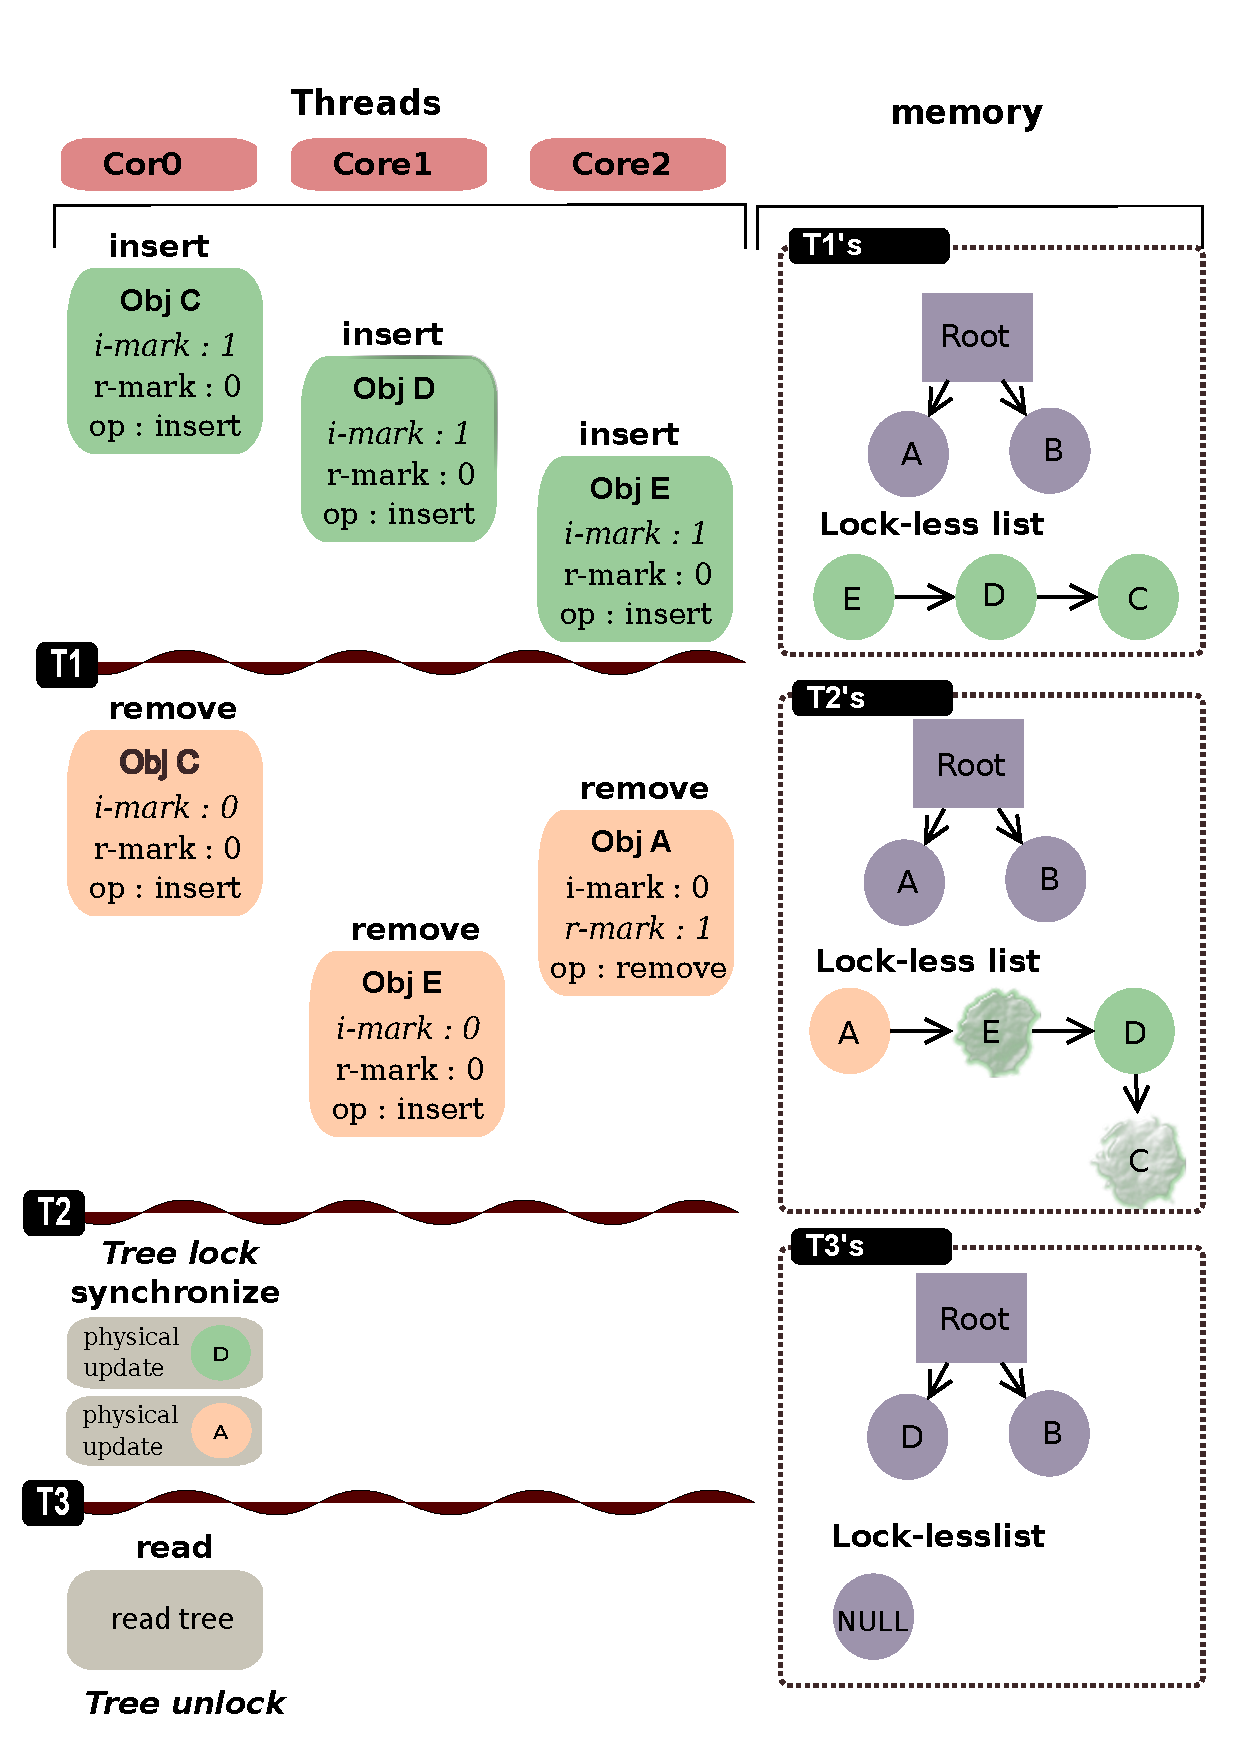
\includegraphics[width=0.5\textwidth,height=0.5\textheight,keepaspectratio]{fig/basic}
%  \end{center}
%  \caption{\deferu example showing six update operations and one read
%  operation. The execution flows from top to bottom. Memory represents original
%  data structure and logging queue at T1, T2 and T3, respectively.}
%  \label{fig:basic}
%\end{figure}

%\subsection{Approach}

%\deferu's scheme for concurrent update is proposed to overcome limitations
%of Linux kernel where 
%both insert and remove operations must not be invoked concurrently for the same
% object, but reads can be concurrently invoked with update.
%\deferu borrows ideas from Oplog's deferred processing and Harris' marking
% scheme.
%The reason is that Linux kernel's object management scheme differs from
% research-oriented data structure such as the lock-free and wait-free data
% structures~\cite{Harris2001Lockfree}~\cite{Fomitchev2004Lockfree}~\cite{Timnat2012}.
%For example, consider the Harris linked list, an insert operation inserts an 
%integer key into the data structure, but Linux kernel inserts their object link.
%The Linux kernel's list operations do not depend on key value.
%Furthermore, Harris linked list node's constructor can be invoked
%upon the insert function's scope, but Linux kernel's node is created on outside scope.
%In this regard, if duplicated remove operation occur, the Linux kernel may
%fail because their link pointer had been freed from destructor.
%Therefore, if a operation is an insert operation, the after operation must occurs 
%remove operation with regard to same object;the remove must execute after the 
%insert, or insert must execute after the remove.
%It means that updates such as insert and remove must not concurrently occur at
%the same object, but reads can occur concurrently.
%\deferu scheme inspires by this operation sequence, and inherits ideas
%from Oplog's deferred processing and Harris's marking scheme.

%\deferu's scheme for concurrent update inspires by Linux kernel's operation
%sequence.
%For example, consider a linked list in Linux kernel, if a operation is an insert
%operation, the after operation must occurs remove operation because Linux
%kernel's object management scheme differs from research-oriented data structure
%such as the lock-free and wait-free data
%structures~\cite{Harris2001Lockfree}~\cite{Fomitchev2004Lockfree}.
%Linux kernel's list operations do not depend on key value, but their 
%list operations depend on their object.
%These structure are their node's constructor can be invoked upon the insert
%function's scope, but Linux kernel's node is created on outside scope.
%In this regard, if duplicated remove operation occur, the Linux kernel may
%fail because their link pointer had been freed from destructor.
%Therefore, the remove must execute after the insert, or insert must execute
%after the remove.
%It means that updates such as insert and remove cannot concurrently occur at
%the same object, but reads can occur concurrently.
%\deferu scheme inspires by this operation sequence, and inherits ideas
%from Oplog's deferred processing and Harris's marking scheme.

%One important algorithm in our proposed novel concurrent update scheme is
%update-side absorbing operation that cancels duplicated operations for
% optimizations.
%A new remove operation, for example, may cancel an existing insert operation
%with regard to same object, so reader can eventually reads consistent data.
%Even though the Oplog's absorbing operation is invoked by
%read, \deferu's absorbing operation is fully invoked by update, so read-side
%performance is enhanced.

%The basic principle of update-side absorbing is that update uses atomic 
%marking operation for the object's mark field, which allows previous operation
% to cancel.
%For instance, if a new remove operation occurs after insert operation of the
%same object, \deferu does not store this operation in the lock-less
%list; instead, it changes the insert mark field to zero using the CAS.
%This mark is checked later when reading operation occurs and the operation log 
%maintained in the lock-less list is applied to original data structure
% atomically.
%This action may give effective update;however, the inserted operation log has
% remained in the lock-less list, so \deferu's reader checks the mark field
% when they convert operation log to original data structure atomically.

%figure : basic principle 
%Figure \ref{fig:basic} gives an example of deferred update with six update
%operations and one read operation.
%In this figure, execution flows from top to bottom.
%The data structure for \emph{physical update} is a tree, and initial values in
%the tree are node \code{A} and \code{B}.
%In contrast, the data structure for \emph{logical update} is lock-less list.
%In the top figure, \code{Core0}, \code{Core1} and \code{Core2} perform the
%logical insert operation to nodes \code{C}, \code{D} and \code{E},
% respectively.
%The logical inserts set the insert mark, and they then insert their
%nodes into lock-less list.
%In this case, none of the lock is needed because \deferu uses the lock-less
%list;all threads can execute the update concurrently.
%At \code{T1}, the tree contains node \code{A}
%and \code{B} and 
%the lock-less list contains node \code{E}, \code{D} and \code{C}.
%When removing the node \code{C}, the node \code{C}, whose mark field was marked
%by insert, atomically cleans up the insert marked field.
%At \code{T2}, the lock-less list contains nodes
%\code{A}, \code{E}, \code{D}, and \code{C}, and the marking field is zero for 
%nodes \code{E} and \code{C}.
%Before running the \code{synchronize} function, they need to lock the original
% tree's lock using the exclusive lock in order to protect the tree's
% operation.
%The \code{synchronize} migrates from lock-less list node to tree node, each of 
%which is the marked node, so nodes \code{A} and \code{D} are migrated.
%Finally, the tree contains nodes \code{D} and \code{B}, so the reader can read
% eventually consistent data.

%First, removing the cancelable operation at update point, \deferu uses the
% update side absorbing instead of read before absorbing.
%Therefore, read before operations in \deferu are fast because read-side
%absorbing operation is eliminated. 
%One notable difference between Oplog and \deferu is that 
%\deferu uses a light weight global queue with non-blocking synchronization 
%for update logs and eliminates time stamps while Oplog is dependent on 
%per-core logs with time stamps.
%By eliminating the global time stamps(hardware-dependent feature), \deferu is
% not dependent on hardware feature.
%Furthermore, update operations in \deferu are also fast because they use
%efficient update-side absorbing that eliminates traversal finding the
%cancelable operation.
%Furthermore, to optimize the log management and minimize the traversal
% overheads during reading, \deferu applies efficient update-side absorbing
% algorithm instead of read-side absorbing algorithm.

%\subsection{logical update}
%\begin{figure}[tb]
%\begin{obeylines}
%\begin{obeyspaces}
%function \(logical\_insert(obj, root) \):
%~~~If CAS(obj.del\_node.mark, 1, 0) $\ne$ 1:  
%~~~    obj.add\_node.mark $\gets$ 1
%~~~    If test\_and\_set\_bit(OP\_INSERT, obj.exist) $\ne$ true:
%~~~        set\_bit(OP\_INSERT, obj.used):
%~~~        obj.add\_node.op $\gets$ OP\_INSERT
%~~~        obj.add\_node.key $\gets$ obj
%~~~        obj.add\_node.root $\gets$ root
%~~~        add\_lock\_less\_list(obj.add\_node)
%~~~
%~~~
%function \(logical\_remove(obj, root) \):
%~~~If CAS(obj.add\_node.mark, 1, 0) $\ne$ 1:  
%~~~    obj.del\_node.mark $\gets$ 1 
%~~~    If test\_and\_set\_bit(OP\_REMOVE, obj.exist) $\ne$ true:
%~~~        set\_bit(OP\_REMOVE, obj.used):
%~~~        obj.del\_node.op $\gets$ OP\_REMOVE
%~~~        obj.del\_node.key $\gets$ obj
%~~~        obj.del\_node.root $\gets$ root
%~~~        add\_lock\_less\_list(obj.del\_node)

%\end{obeyspaces}
%\end{obeylines}
%\rule{\columnwidth}{0.5pt}
%\vspace{-\baselineskip}
%\caption{\deferu logical update algorithm. \code{logical\_insert} represents
% non-blocking insert function.
%It may be called by original insert position without locks. The fastpath is
% that when their object was removed by \code{logical\_remove},
% \code{logical\_insert} just changes node's marking field.}
%\label{fig:logicalupdate}
%\end{figure}

%The pseudo code for \deferu's \emph{logical update} is given in
%figure~\ref{fig:logicalupdate}.
%The \code{logical\_insert}, the concurrent update function, checks whether this
%object already has been removed by \code{logical\_remove}.
%If this object has been removed, \code{logical\_insert} initializes the marking
% field and then they return, which is fastpath.
%The marking field needs synchronization because this field in the
%\emph{logical update} is shared with the \emph{physical update}, so the CAS
% operation is needed.
%When the marking field has been initialized, they set the
%marking field, then they check whether or not this node already has been
% inserted in lock-less list.
%If the node does not exist in lock-less list, then they insert the node into
%lock-less list.

%\subsection{Physical update}
%\begin{figure}[tb]
%\begin{obeylines}
%\begin{obeyspaces}
%function \(synchronize\_ldu(obj, head) \):
%~~~If (head.first = NULL): 
%~~~    return; 
%~~~entry $\gets$ xchg(head.first, NULL);
%~~~for each list node:
%~~~    obj $\gets$ node.key
%~~~    clear\_bit(node.op, obj.exist)
%~~~    If CAS(node.mark, 1, 0) = 1:
%~~~         physical\_update(node.op, obj, node.root)
%~~~    clear\_bit(node.op, obj.used)
%~~~
%function \(physical\_update(op, obj, root) \):
%~~~If op = OP\_INSERT :  
%~~~    call real insert function(obj, root) 
%~~~Else If op = OP\_REMOVE :  
%~~~    call real remove function(obj, root) 

%\end{obeyspaces}
%\end{obeylines}
%\rule{\columnwidth}{0.5pt}
%\vspace{-\baselineskip}
%\caption{\deferu physical update algorithm. \code{synchronize\_ldu} may be
% called by reader and converts update log to original data structure
% traversing the lock-less list.}
%\label{fig:physicalupdate}
%\end{figure}

%The pseudo code for \deferu's \emph{physical update} is given in
%Figure~\ref{fig:physicalupdate}.
%First, they check whether lock-less list is an empty list or not, then they
%iterate the lock-less list.
%If the marking field has been set, they execute migration from
%lock-less to original data structure.
%Because the marking field in \emph{physical update} is shared with
% \emph{logical update}, the CAS operation is needed.
%They initialize the used field, which needs to protect the object from freed
% through destructor.
%The programmer must acquire locks on the \code{synchronize\_ldu} function,
%which migrates log to original data structure.
%Finally, the \code{physical\_update} executes original functions by using the
%operation log.
